\documentclass[UTF8]{ctexart}

\usepackage{geometry}
\usepackage{hyperref}
\usepackage{graphicx}
\usepackage{appendix}
\usepackage{adjustbox}

\geometry{a4paper,scale=0.8}

\title{
  电影数据分析与电影推荐模型\\
  \large 人工智能引论实践课作业报告}
\author{张开 1800012977 \ 张屹洋 1800013111 \ 郑钦源 1800013003}

\begin{document}

\maketitle
\tableofcontents
\newpage

\section{作业要求}
\par 根据给定的TMDB 5000 Movie Dataset\footnote{\href{https://www.kaggle.com/tmdb/tmdb-movie-metadata}{https://www.kaggle.com/tmdb/tmdb-movie-metadata}},完成以下任务:
\begin{itemize}
  \item 电影数据分析及可视化
  \begin{itemize}
    \item 各类型电影分布
    \item 各类型电影数量随时间的变化
    \item 电影关键词分析
  \end{itemize}
  \item 电影推荐
  \begin{itemize}
    \item 基于内容
    \item 协同过滤
  \end{itemize}
  \item 电影分数预测
\end{itemize}

\section{需求分析}
\par 综合分析作业要求以及给定数据,我组更倾向于对数据进行一定处理后进行主观分析以及对实际问题进行建模。考虑到选择该课题的小组数量,以及对于电影推荐、评分等存在的主观性,难以形成统一的评判标准,因此我组希望在给出一个可靠模型的基础上,再给出一个相对完善的系统以方便主观评判。
\par 鉴于电影数据分析与可视化部分要求了基于时间的分析,最好能有一定的自定义能力(动态调整展示时间段等);又电影推荐、电影分数预测部分需要给出部分信息并展示结果,我组最终决定同时开发一SPA\footnote{Single Page Application.}作为用户交互的渠道。
\par 此外,经过对给定csv文件的分析,我组发现其中有相当一部分数据域本质上是以JSON格式给出,而JSON里的不同对象均已与独一无二的ID对应好。为了方便后续数据处理以及加快数据查询速度,我组决定使用某种数据库进行管理。

\section{实验方法与结果}
\par 整体的实验结果展示、试用系统参见\href{http://104.248.157.18:3000/}{http://104.248.157.18:3000/}。
\subsection{基础准备}
\par 为尽可能快的开发该SPA,将重点放在数据分析与建模上,我组决定使用相对成熟的Nuxt.js\footnote{\href{https://nuxtjs.org/}{https://nuxtjs.org/}}作为整体框架。数据可视化部分,使用生态良好、功能丰富的Echarts\footnote{\href{https://echarts.baidu.com/}{https://echarts.baidu.com/}}开发;其余部分各组员分工,由Node.js后端统一处理子程序的交互。
\par 数据库方面,我组使用了开源的MariaDB\footnote{\href{https://mariadb.org/}{https://mariadb.org/}}管理。提取出本作业需要且与电影具有多对多关系的域有:
\begin{itemize}
  \item{genre} 类型
  \item{keywords} 关键词
  \item{production\_companies} 制片公司
  \item{cast} 演员
  \item{crew} 职员
\end{itemize}
\par 对电影与这些域各自建立数据表,并建立关系表以存储电影与其他域的关系。

\subsection{电影数据分析及可视化}
\par 由于已经将数据预处理,因此只需在数据库中查询需要的信息直接递送给Echarts实例即可。以下为对结果的分析。
\subsubsection{各类型电影分布}
\par 数量排名前五的电影类型为:Drama-剧情,Comedy-喜剧,Thriller-惊悚,Action-动作,Romance-浪漫。这和我们对电影的普遍认知相符合。
\begin{figure}[ht]
  \centering
  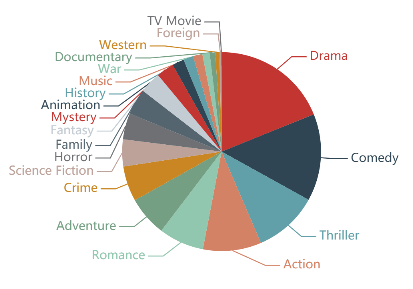
\includegraphics[scale=.5]{distribution.png}
  \caption{Genre Distribution}
\end{figure}
\subsubsection{各类型电影数量变化}
\par 这部分我们以5年为跨度进行分析。早期电影数量不多,每五年有大约几十部电影发行,但类型已经比较多样化;从1970年左右,每半旬电影数量突破100;在1990年,电影数量开始井喷式增长,其势头一直持续到2005年,其后的电影数量反而下降。其原因可能是电影市场确实达到了饱和,但更可能是该数据库本身进行了一定筛选,并没有完全覆盖所有近年来发行的电影。从各个类型分析,浪漫、犯罪、悬疑等曾经比较火热的类型似乎已经难以让人们提起兴趣,反而是惊悚、动作、科幻有仍走高态势。不难推断,随着信息技术的发展,电影后期特效的制作水平已经可以达到非常高的水平,通过特效营造情景氛围,让观众更有代入性、大呼过瘾的同时,也更喜欢观看这样的电影,促进了这些类型电影的发展。此外,通过特效营造的奇幻世界突破了传统拍摄手法的局限,让艺术家的想象力能在更广阔的空间畅游,更为自由地表现其天马行空的创意。另一点值得注意的是,同样上升的还有经久不衰的音乐剧与动画。我们推断,随着物质生活水平的提高,人们也有提高精神生活水平的需求。音乐与动画作为更加传统的艺术表现形式,其间佳作频出,同样有效形成了正反馈。
\begin{figure}[ht]
  \centering
  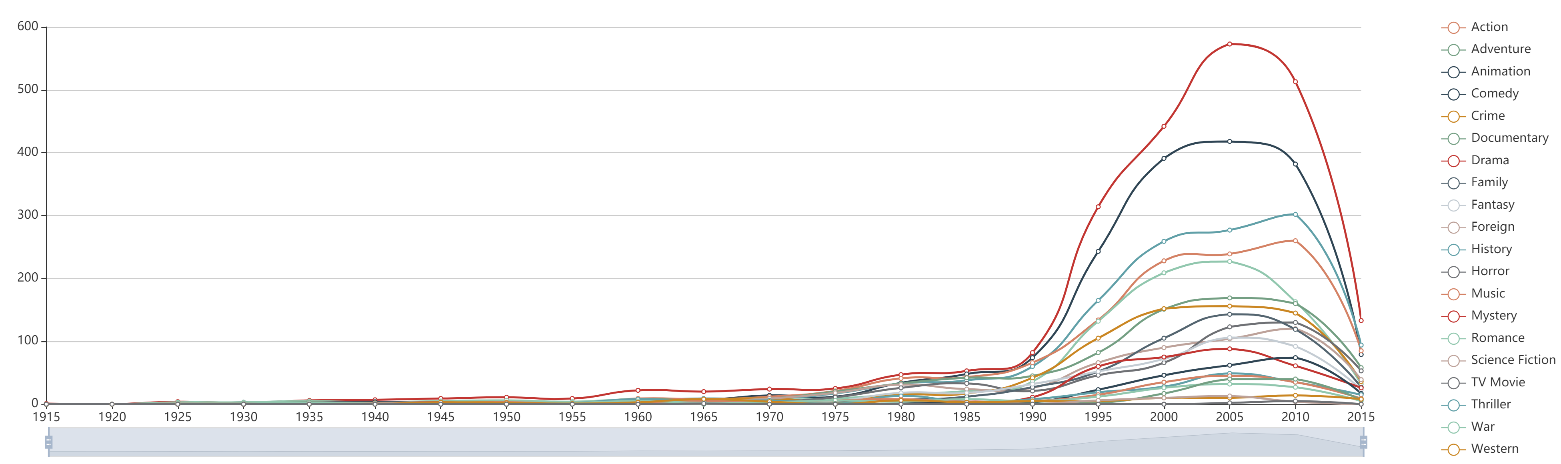
\includegraphics[scale=.3]{trend.png}
  \caption{Genre Trend}
\end{figure}
\subsubsection{电影关键词分析}
\par 数据中最早的电影出现在1910年代,而1910-1930年间占比最大的关键词即为“默片”(Silent Film)。有趣的是,早在那是已经有诸如“机械城市”(Machine Town)“人 VS 机器”(Man VS Machine)等对未来的想象,代表作品包括1927年的《大都会》(\textit{Metropolis})。之后影片配上了声音,就出现了“音乐剧”(Musical),相伴的关键词还有“舞蹈”(Dance)“表演”(Stage Show)等。电影作为一种新的艺术形式,逐渐走进了人们的生活。
\par 1940年代出现最多的关键词是“黑色电影”(Film Noir)。这个不太常见的关键词主要指“好莱坞侦探片”,特别是强调愤世嫉俗,或出于性动机的题材。这写电影的取材很多出自于大萧条时期的硬汉文学,也与战时、战后现实的幻灭有一定的关联。而战争一直是人们经久不衰的话题与灵感源泉。1960年代,在词云图中最为显眼的几个关键词包括“秘密组织”(Secret Organization)“英国”(England)“二战”(World War II)“冷战”(Cold War)“士兵”(Soldier)……但虽然如此,几部非常有代表性的电影却没有在其中表现出来,如《惊魂记》(\textit{Psycho})《音乐之声》(\textit{The Sound of Music})《2001太空漫游》(\textit{2001: A Space Odyssey})等。电影的多样性,此时仅靠关键词已经很难估量。
\par 1970年代的关键词是“反乌托邦”(Dystopia)。也许出于对哲学与社会的思考,人人向往的乌托邦社会,往往与现实相背离,而有了电影这种更为形象的艺术表现形式,艺术家们对于极端恶劣的社会形态得以表现,譬如《发条橙》(\textit{A Clockwork Orange})中对于人性善恶的考量……与此同时出现的另一个关键词是“独立电影”(Independent Film),并持续多年占据词云图。随着技术的发展,简单的电影拍摄成本不断降低,这也带给了更多人不依赖于公司扶持,自己组建团队拍摄电影的机会。越来越多的导演开始展现自己的创造力,这也让电影艺术能够不断开花结果。同期的另一个关键词“女导演”(Woman Director)大概也说明,性别平权意识的涌动。
\par 21世纪的主要关键词却是“彩蛋”(Stinger),还分为During Credits和After Credits两种。作为一个与电影内容基本不相关的关键词,其实是为了电影增加了一些趣味性——也吊人胃口。漫威世界的太多部电影着实为这个关键词贡献了很大的权重。

\subsection{电影推荐}
\subsubsection{基于内容}
\par 对于电影推荐功能的实现,我组的基本思路是基于用户的自由输入给出能让用户满意度最高的前10部电影。用于评价这一指标的关键因素是输入与电影属性的相似和匹配程度。综上,这一部分主要做的是对于输入和信息的匹配。
\par 对于电影的演职员、类型以及制片公司,它们都是特定的离散特征,直接进行匹配即可,匹配程度越高的电影,分配越高的权重。而电影推荐部分中最不可缺少的,最重要的也是最难处理的部分其实是关键词(keyword)筛选。鉴于自然语言的复杂性,数据库给出的关键词列表中关键词很可能与用户输入的关键词不完全匹配,而互为同义词或近义词,或词形不同而导致无法直接匹配。查阅一些资料后,我们使用了NLP中非常常用的NLTK库\footnote{\href{https://www.nltk.org/}{https://www.nltk.org/}}。因此,我组基本思路为扩展用户输入和数据库提供的关键词为它们同义词根的集合,然后寻找交集。具体而言,对于数据库给出的每个关键词,利用NLTK Corpus中的Wordnet,扩充为其同义词的集合(为了防止过扩充,指定每个词最多扩充为5),并通过stem模块处理出词根存储,记为电影的关键词特征。在进行关键词匹配的时候,对于用户输入的关键词集合进行相同的操作,得出扩充后的词根集,再和每部电影的关键词特征取交集,计算匹配个数即可。
\par 其后是对于综合推荐指数的计算。简单的匹配个数直接线性求和的方式可能会导致权重失衡,即出现一个特征匹配完全但其他特征不匹配时产生较大权重的情况。我组使用三重优先级排序的策略,排序顺序为:
\begin{enumerate}
  \item 用户的所有输入是否都得到了一定程度的满足
  \item 用户的输入得到一定程度满足的数量
  \item 匹配个数
\end{enumerate}
\par 此外,我们对于这些推荐指标使用电影的综合评分(vote\_average)进行加权处理,使得在大众中口碑较好的电影可以优先被推荐。为防止评分样本过少产生的偶然性,我组也参考数据中给出的评分数量(vote\_count),对于评分人数过少的电影进行一定比例的减分,也减少冷门电影的推荐。而票房(revenue)、流行度(popularity)等特征在一定程度上同样反映了电影的受欢迎程度,因此分别加适当的权值处理。最后,使用上述的三重优先级排序,将排名前十的电影推荐给用户。
\subsubsection{协同过滤}
\par 协同过滤主要是基于“人-物-关联”的数据信息来寻求“人-人”或“物-物”的联系,从而达到优质推荐的目的。作业要求自行寻找用户评分数据,幸运的是,网络上有包含了很多TMDB电影用户评分的MovieLens数据集\footnote{\href{https://grouplens.org/datasets/movielens/}{https://grouplens.org/datasets/movielens/}}。为尽可能覆盖已有数据集中电影,我组选用ml-latest数据集,并从中筛选出包含在已有数据库中的电影;均衡考虑,按用户排序后使用了前$10^6$条数据。
\par 处理好数据后,面对形式为“用户-电影-评分”关系,基于不同对象,有两种选择:
\begin{itemize}
  \item{基于用户} 寻求用户之间的关联。以两个用户对各部电影给分的一致与否作为关联的标准,用数据库生成用户形象分类。进行推荐时,系统根据输入的电影生成当前的用户形象,并用户形象类别中进行匹配,最后返回该类普遍给分较高的电影;
	\item{基于电影} 寻求电影之间的关联。通过两部电影获得各用户给分的一致与否作为关联标准,用数据库生成“电影-电影”的关联度矩阵。进行推荐时,系统根据输入的多部电影寻求各自关联度最高的多部电影,最后进行综合排序取优。
\end{itemize}
\par 然而协同过滤也有它的局限性,不能只靠它来进行推荐:由于用户对电影的评价很大程度与影片质量有关,因此质量相近但风格迥异的电影很有可能也会收获相近的评分,而生成的用户类群也会不甚明晰。因此我们选择先“以物为本”,把第一种“基于内容”评价方式中的数据进行再加工,将“电影-电影”内容属性的相似度提炼出来作为匹配的硬性标准;然后再利用协同过滤这个强有力的人性化推荐手段,让推荐结果不受限于标签和属性的计数,更受到由真人用户给出的“用户-电影-评分”数据的影响。
\par 因此我有如下的实践步骤:
\begin{enumerate}
  \item 利用“用户-电影-评分”数据计算出了每个用户的平均打分,再将某个用户对某个电影的评分减去该用户的平均给分,作为该用户对该电影的喜好程度,从而矫正每个用户总体打分偏高或偏低带来的评分误差。
  \item 我们对每两部电影进行分析,将两者共有的打分用户作为参照,把每个用户的给分作为一个维度,在生成的空间中计算两部电影对应的向量夹角,作为协同过滤生成的两部电影的关联度。
  \item 在处理“基于内容”评价方式所得数据库时保留每部电影关联度最高的$40$部电影,再对这个$5000\times 40$的“电影-电影”矩阵中的每个关联度添上我们通过协同过滤所得到的相应“电影-电影”关联度,最终进行关联度的求和、排序,即可得到推荐的电影。
\end{enumerate}
\par 关联度使用如下公式计算:($R_{um_i}$:用户$u$对电影$m_i$的评分;$R_u$:用户$u$的平均给分)
$$ sim(m_1,m_2)=\frac{\sum_u{(R_{um_1}-R_u)(R_{um_2}-R_u)}}{\sqrt{\sum_u{(R_{um_1}-R_u)^2}\cdot {\sum_u{(R_{um_2}-R_u)^2}}}} $$

\subsection{评分预测}
\par 该问题可视为给定某些输入后的回归问题。而对于给定输入的范围,我组做了如下考量:
\begin{itemize}
  \item{budget, releaseYear, revenue, runtime} 为数值,常识上可供参考
  \item{cast, crew, genre, productionCompany} 为固定离散量,常识上可供参考
  \item{keyword} 为固定离散量,但难以让用户输入限制在定义域内,参考意义不大
  \item{language} 93.8\%电影为英语,参考意义不大
  \item{homepage, overview, tagline, title} 纯文字信息,参考意义不大
\end{itemize}
\par 因此我组决定要求用户提供上述可供参考量,并通过已有数据训练深度神经网络以预测评分。
\par 对于预算和票房,往往数值过大,为不产生太大的影响,将其统一除以$10^5$后同发行年份和片长作为4个输入节点。
\par 对于离散变量,由于定义域过大,因此将变量信息经过另一组神经网络计算后压缩为15个节点,同数值变量的4个节点一起构成主体神经网络的64个输入节点。之后通过若干全连接层,归结为一个输出节点。
\par 但对于演职员来说,超过$10^5$的取值范围仍然太大,无法保证训练准确性,而且极大地增加了训练复杂度。因此对于演职员和制片公司,各自寻找一个$k$,使得在$k$部以上电影中出现的值的种类数不超过$2000$,也因此限制使用的变量取值,对于其他一律舍弃。对于每个离散变量,将取得的值置为$1$,其他置为$0$,作为该部分神经网络的输入,经过带有softmax激活函数的全连接隐藏层后再进行比例为0.3的Dropout,输出15个节点作为主神经网络的输入。(图 \ref{fig:model})
\newpage
\begin{figure}[ht]
  \centering
  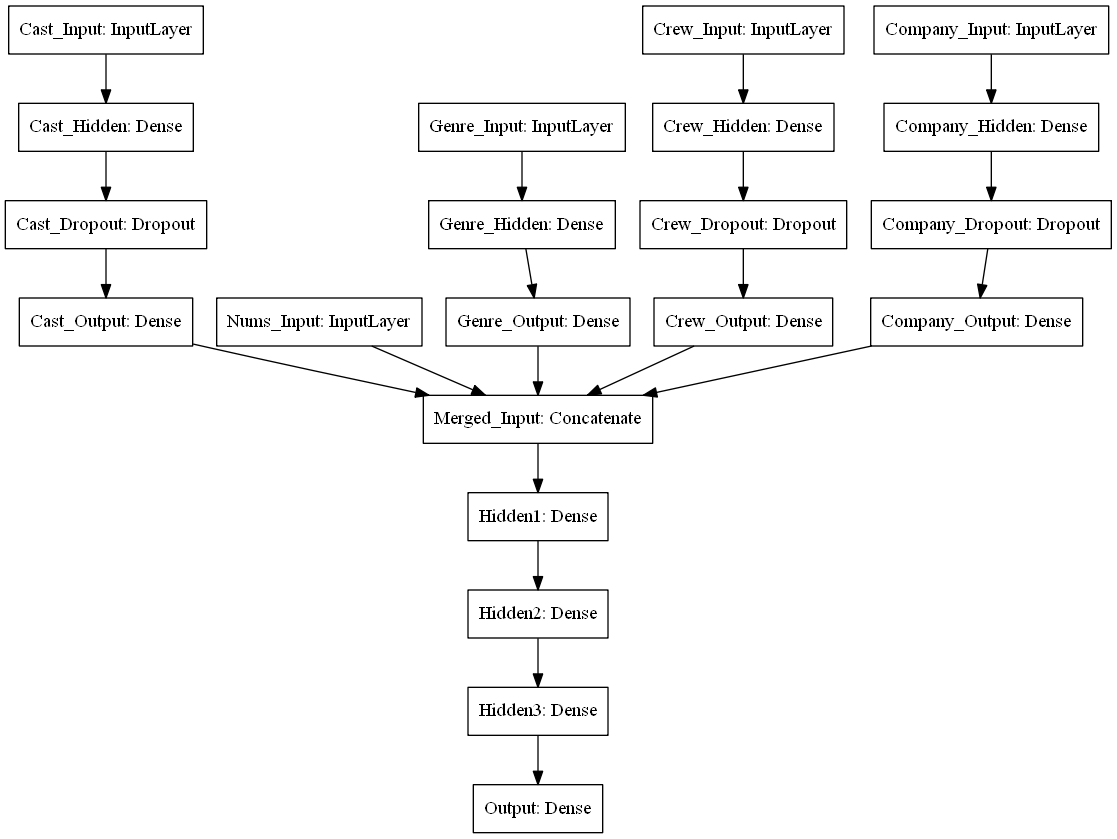
\includegraphics[scale=.4]{model.png}
  \caption{NN Model}
  \label{fig:model}
\end{figure}
\par 设置50的耐心度后,训练在大约440个epoch后提前停止,此时从所有数据中随机抽取出的10\%测试集上MSE Loss约为0.7,即与实际评分差异均值约为0.8,相对而言可以接受。而在TMDB上选取的若干新电影上的测试,具有相似表现,因此可以认为是可接受的训练结果。
\par
\centering
\begin{tabular}{cccc}
\hline
TMDB ID& Title& Real Rating& Forecast\\
\hline
447404& Pokémon Detective Pikachu& 7.0& 6.12\\
299534& Avengers: Endgame& 8.5& 8.31\\
284052& Doctor Strange& 7.3& 7.57\\
313369& La La Land& 7.9& 7.20\\
274870& Passengers& 6.8& 6.75\\
\hline
\end{tabular}
\section{总结}
\par 通过本次作业,我组同学了解并参与实践了实际的数据处理、挖掘工作,也接触了如数据库管理、协同过滤算法、神经网络等比较成熟可靠的方法,经历了一次“小科研”,可以说是收获颇丰。但仍有一些可以提升的空间,如尝试从电影中挖掘更多信息,进一步调整神经网络结构以达到更好效果,查阅参考前任文献资料等。相信有了这次宝贵经验,我们会在以后的工作中做得更好。

\end{document}